Thinking...
We need to translate the Japanese sentence into English, preserving TeX code unchanged. The Japanese sentence: "以下のの日本語文を英訳してください。ただしTeXのコードが挿入されているのでその部分はそのまま出力してください：" then the TeX figure environment. So we need to translate the Japanese instruction? Actually the user says: "以下のの日本語文を英訳してください。ただしTeXのコードが挿入されているのでその部分はそのまま出力してください：" then provides the TeX code. So we need to translate the Japanese text within the caption? Actually the caption is Japanese: "高被引用論文に付与された高被引用テーマの種数". So we need to translate that caption into English while preserving the surrounding TeX code unchanged. The rest of the TeX code should remain same. So output should be the same LaTeX environment but caption translated.

Thus we output:

\begin{figure}[h]
\begin{center}
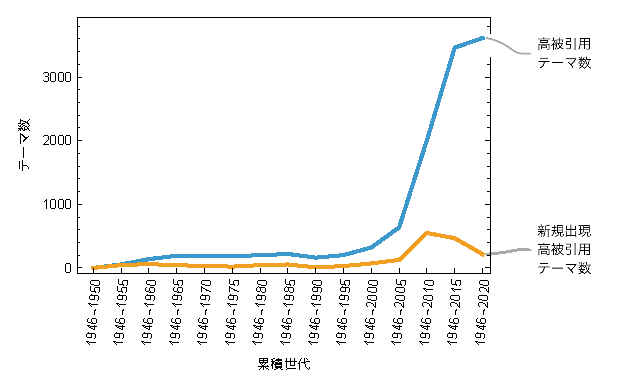
\includegraphics[width=76mm]{gr13.eps}
\caption{Number of distinct highly-cited themes assigned to highly-cited papers}
\label{fig:gr13}
\end{center}
\end{figure}

We need to ensure no extra modifications. Probably also translate "高被引用論文に付与された高被引用テーマの種数" accurately: "Number of types of highly-cited themes assigned to highly-cited papers". Could phrase as "Number of distinct highly-cited themes assigned to highly-cited papers". That is fine.

Thus output only the TeX block with translated caption.
...done thinking.

\begin{figure}[h]
\begin{center}
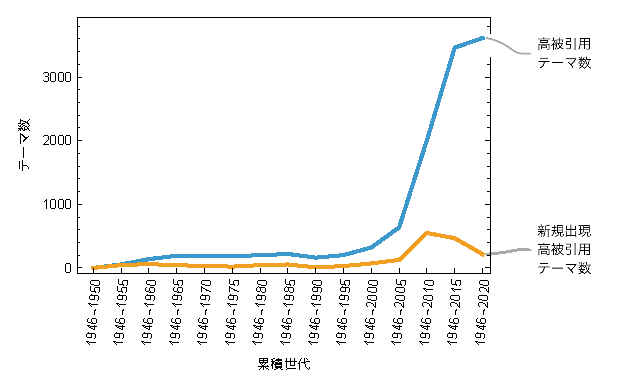
\includegraphics[width=76mm]{gr13.eps}
\caption{Number of distinct highly‑cited themes assigned to highly‑cited papers}
\label{fig:gr13}
\end{center}
\end{figure}

